\pdfminorversion=7
\documentclass[../main.tex]{subfiles}

\begin{document}
\ifx\chapincluded\undefined
  \begin{refsection}[main-bib]
 \fi

\chapter{Background}
\label{chap:background}

%Paper giving background on serverless computing \cite{van2018serverless}

% \subsection{Designing a Microarchitecture for the Datacenter}

\section{Instruction Delivery in the Datacenter}
\label{sec:instr-delivery}

% TODO: This was inteded to be a separate sectoin on the BTB but for now it just points here
\label{sec:btb-background}


% Front-end problem -> what people have done
Datacenter workloads are distinguished by having massive multi-megabyte instruction footprints. These workloads generally have deep, multi-layered software architectures with deep dependency stacks. For example, a request hitting a website invokes the web server, the interpreter of the backend language powering the website and a database server. All of these components also involve a large amount of system calls that perform context switches and execute a significant amount of kernel code. footprint~\cite{ferdman12_clear_cloud,ailamaki99_dbmss_moder_proces}. These large code footprints overwhelms the capabilities of the frontends of common processors causing a phenomenon known as the front-end bottleneck~\cite{kanev15_profil,ferdman12_clear_cloud,ayers19_asmdb,kanev15_profil,kumar17_boomer,kumar18_blast_throug_front_end_bottl_with_shotg,kumar20_shoot_down_server_front_end_bottl,spracklen05_effec_instr_prefet_chip_multip}.



The front-end bottleneck occurs when the frontend of the processor is
unable to deliver a contiguous stream of instructions to the
backend.
% Write about what happens when the pipeline fills an instruction
For every Instruction delivery interruptions from the front-end can
occur for two reasons: \begin{inparaenum}[1)] \item the frontend
  mispredicts the next instruction due to a branch misprediction or a
  branch target miss or \item the frontend encounters a L1-I
  miss.\end{inparaenum}. Recovering from either of these events is
extremely expensive due to an extensive number of pipeline stall
cycles where the processor core is prevented from making
progress. When a branch misprediction occurs, the execution core must
be resteered onto the right-path execution. Doing this requires a
pipeline flush, exposing the core to a pipeline fill latency of tens
of cycles. L1-I cache misses are even more expensive exposing the core
to the cache fill delay occurring while the right-path instruction is
loaded into the cache.

Traditionally, the instruction cache prefetching capabilities of
processor frontends consisted of only next-line prefetching
(NLP)~\cite{nextline_pref}. In NLP, the next instruction cache block
is prefetched unconditionally. While this provide effective coverage
for linear code execution in covering the discontiguous control flows
with large spatial footprints that are common in server processors. To
address this, researchers has proposed diverse hardware mechanisms for
instruction prefetching. We generally subdivide these into two
categories: temporal streaming and fetch-directed prefetching. We describe these in the following

\paragraph{Temporal Streaming.} Fundamentally, temporal streaming
based prefetching exploit the repetitiveness of program control
flow. The intuition behind this is that even is a program can perform
several operations, the instruction sequence executed to perform each
operation is similar. This principles enables instruction prefetching
through a record and replay approach, where streams of instructions
are recorded and subsequently and replayed when a prerecorded pattern
of instruction accesses is seen. \textcite{ferdman08_tempor} proposed
Temporal Instruction Fetch Streaming (TIFS), the original prefetcher
exploiting this principle. While TIFS is effective at avoiding
instruction cache misses it requires a massive amount of metadata
storage to capture the recorded streams.  Proactive Instruction
Fetch~\cite{ferdman11_proac_instr_fetch} improves on both the performance and metadata storage requirements of TIFS by recording compacted retire-order instruction streams. Still, it requires large amounts of metadata storage of 200KB per core.
\truls{Describe other temporal streaming approaches}

To summarize, prefetchers based on temporal streaming are highly effective at eliminating L1-I misses but they do so at the cost of requiring large amounts of metadata storage and complex dedicated logic.

\begin{figure}[ht]
  \centering
  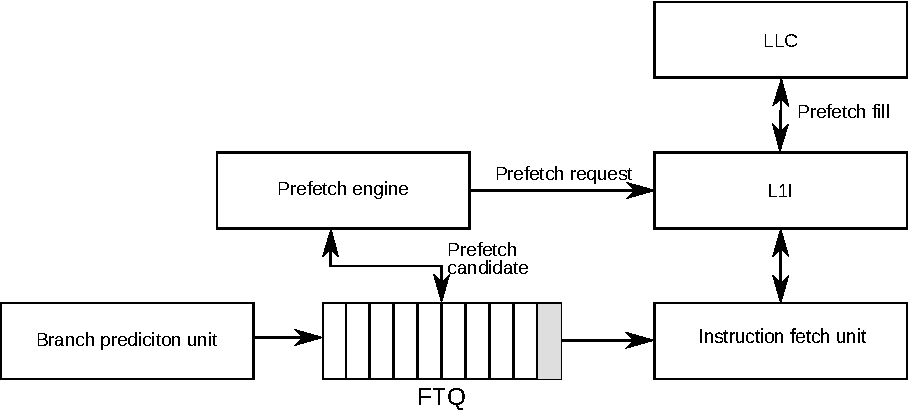
\includegraphics[width=0.8\textwidth]{figures/fdip1.pdf}
  \caption{\label{fig:fdip} A schematic of the FDIP architecture.}
\end{figure}

\paragraph{Fetch-directed prefetching}
The Branch Target Buffer (BTB) has several important roles in a modern high-performance processor

\textcite{reinman99_fetch_direc_instr_prefet} proposed a prefetching
mechanism known as Fetch-Directed Instruction Prefetching (FDIP). The
key insight of FDIP is that since the BTB holds branch targets in a
program, it already contains the metadata needed for prefetching. A
schematic of FDIP is shown in\Cref{fig:fdip}. FDIP decouples the
branch prediction unit form the fetch unit using a dedicated queue
known as the Fetch Target Queue (FTQ). This decoupling allows the
branch prediction unit to run ahead of the program execution and fill
the FTQ with locations of future predicted control flow. Thus, the
targets in the FTQ represents ideal instruction cache prefetch
candidates since they represent future control flow of the program
being executed. In spite of FDIP's alluring simplicity and requiring
zero additional metadata, conventional wisdom long held that FDIP, and
fetch-directed prefetchers in general, wer incapable of effectively
covering instruction cache misses in commercial server workloads. One reason for this 




Be sure to explain how the BTB impacts instruction delivery by aiding FDIP-backed instruction prefetching.



% \cite{kanev15_profil,ferdman12_clear_cloud}

% \subsubsection{The Branch Target Buffer}

%Two prefetching approaches: FDIP and streaming

% FDIP approaches: \cite{reinman99_fetch_direc_instr_prefet, kumar17_boomer,kumar18_blast_throug_front_end_bottl_with_shotg,kumar20_shoot_down_server_front_end_bottl}

% Streaming approaches:
% \cite{ferdman08_tempor,ferdman11_proac_instr_fetch,kaynak13_shift,kaynak15_confl}

% Profiling based:

% RDIP-based methods are superior but require highly-efficient prefetchers to work. This motivated the development of BTB-X

% Explain diffeernt approaches, prefetching, BTB, cache replacement

% Add a description of the processor frontend

\section{Serverless Computing}

Communication problem -> what people have done

% \subsection{Serverless computing: Characteristics and challenges}
% \label{sec:serverless}
% Serverless is cool, attractive and highly used. What are the characteristics and challenges that makes it unique?

% Mention cold start latency

\section{Serverless Computing and the Front-end Bottleneck}

\ifx\chapincluded\undefined
  \printbibliography
  \end{refsection}
 \fi
\end{document}

%%% Local Variables:
%%% mode: latex
%%% TeX-master: t
%%% TeX-command-extra-options: "-shell-escape"
%%% End: